\documentclass[a4paper]{article}

\usepackage[utf8]{inputenc}
\usepackage[T1]{fontenc}
\usepackage[francais]{babel}
\usepackage{geometry}
\usepackage{graphicx}

\title{\Huge \textbf{Rapport de projet tuteuré}}
\author{\Large Felton - Gros - Impéras - Piat - Vareille}
\date{15 Janvier 2015}

\begin{document}

\maketitle
\newpage

\tableofcontents
\newpage

\section{Cahier des charges}
	\subsection*{Introduction}
	
	Pour ce deuxième semestre, la réalisation d'un site dynamique est demandée. A l'unanimité, le choix du sujet fût rapidement décidé : un site proposant la vente et la réservation de voiture ainsi que d'accessoires automobiles. Il est aussi envisagé de mettre à disposition du gérant une application graphique afin de simplifier diverses tâches.
	\subsection{Précision du domaine}
	
	Plusieurs gammes de véhicules seront proposées, selon les besoins, les moyens et les attentes du client. Du véhicule utilitaire à la citadine en passant par des deux roues, le site ne fera aucune exception. Quant au public visé, aucune restriction n'est envisagée. Jeunes conducteurs, routiers ou professionnels recherchant des véhicules appropriés.
	
	Un achat direct de véhicule ne sera pas disponible directement via le site, un devis personnalisé sera généré et un rendez-vous réel sera programmé avec le vendeur.
	
	En plus de cela, des accessoires pour véhicule en tout genre seront disponibles à la vente.
	
	Le gérant peut ajouter un nouvel article grâce à l'application, en rentrant toutes les informations concernant le produit. Il peut aussi visualiser les divers clients, ainsi que leurs dernières commandes.
	
	Le client, en naviguant, peut visualiser toutes les informations concernant le produit, Il peut par exemple voir la marque du produit et ses différentes spécificités. 
	\subsection{Besoins d'utilisateurs}
		\subsubsection{Besoin du client}
	Sur le site, l'utilisateur aura accès à plusieurs fonctionnalités, répondant à des besoins particuliers.
	
	Trouver un moyen de locomotion et des accessoires liés à ce dernier.
	En effet, guider la navigation et l'adapter en temps réel à chaque réitération de la recherche est quelque chose de primordial. 
	
	Un aperçu du prix d'une commande via différentes techniques (panier, devis etc.) est une étape importante pour instaurer une confiance de la part du client.
	
	En cas de commande réalisée, un historique précis et détaillé sera disponible à la consultation via un espace personnel propre à l'acheteur.
	
	Trouver simplement des informations sur les produits présentés ainsi qu'effectuer des recherches rapides et précises. 
	
	L'utilisateur aura un compte personnel, après avoir rempli le formulaire d'inscription. Lors de son achat (voiture ou accessoire), il sera prié de se connecter afin de finaliser sa commande. S'il n'est pas déjà inscrit, il en sera prié.
	
		\begin{figure}[t]
		\centering
			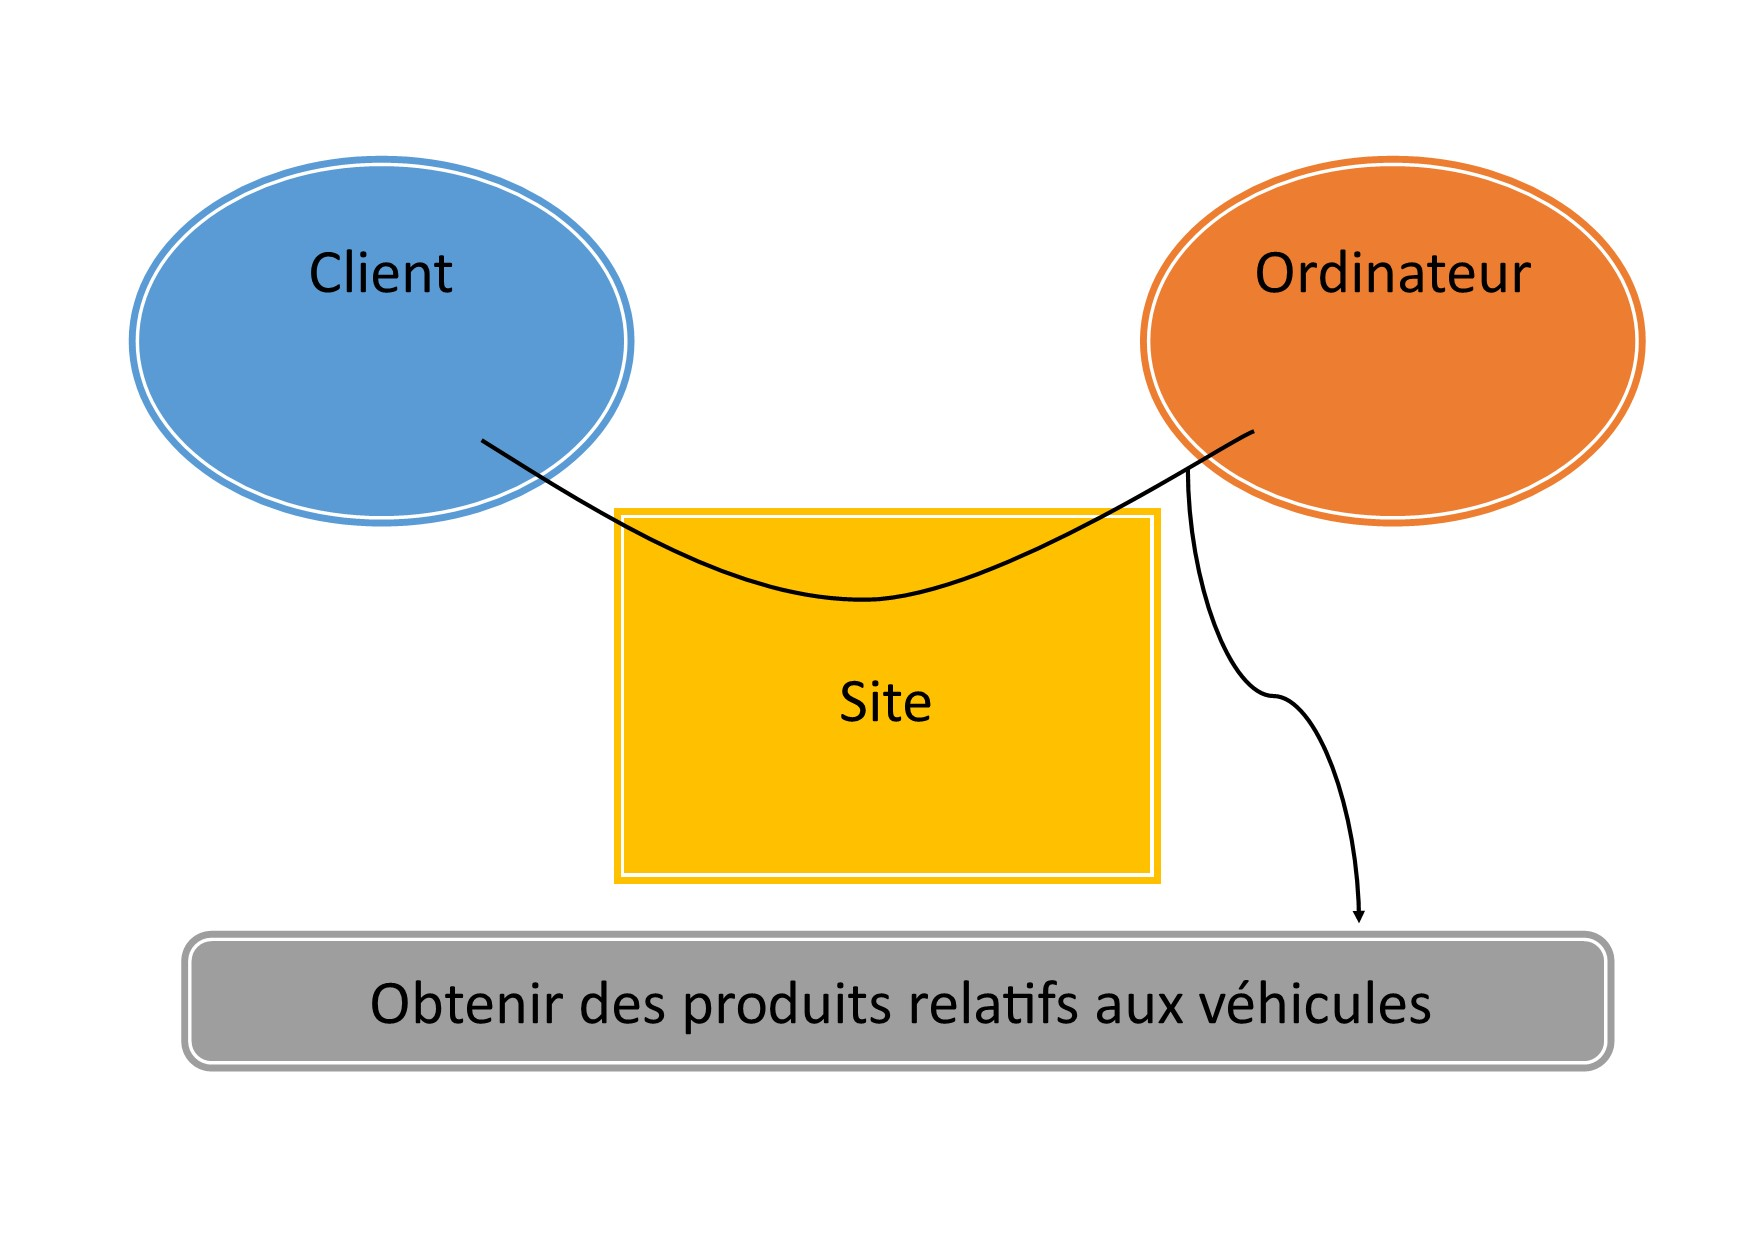
\includegraphics[scale=0.5]{../graph/beteACorne1.jpg}
			\caption{Diagramme des prestations client (ou Bête à corne)}
	\end{figure}
		\newpage
		\subsubsection{Besoin du vendeur}
		L'utilisation du site lors d'une connexion via un compte vendeur ne sera bien évidemment différente que lors d'une connexion cliente.
		
		La gestion des stocks ainsi que l'ajout de nouveaux produits seront des options disponibles. Il faut pouvoir en temps réel les capacités du stock, afin qu'un client ne puisse pas commander un produit en rupture de stock.
		
		Il faudra également procéder à l'enregistrement des ventes, ainsi que la gestion des clients (telle que la visualisation des informations pour chaque utilisateur, etc...).
	
	\begin{figure}[!t]
		\centering
			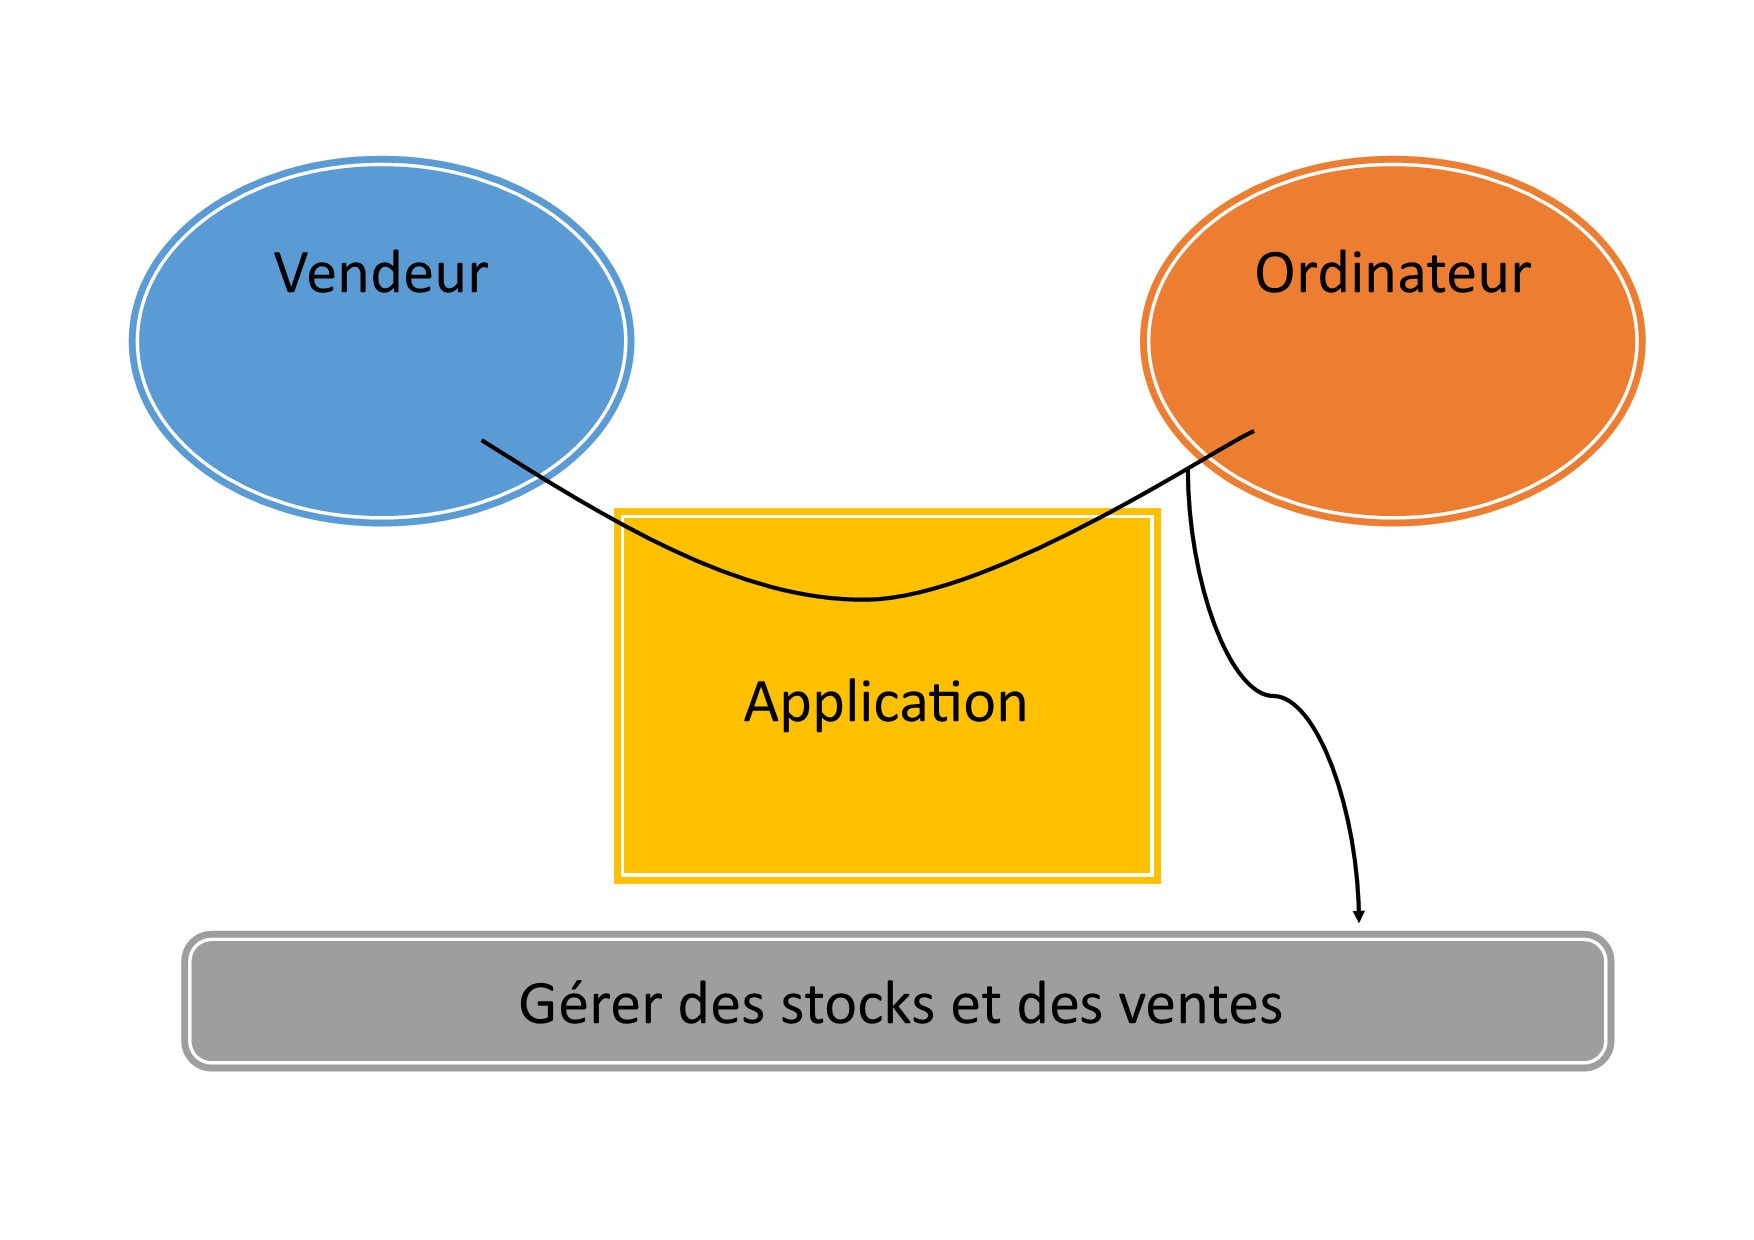
\includegraphics[scale=0.5]{../graph/beteACorne2.jpg}
			\caption{Diagramme des prestations vendeur (ou Bête à corne)}
	\end{figure}
	
	\newpage
	~ 
	\newpage
	\subsection{Spécifications fonctionnelles}
	\begin{itemize}
		\item[]{Failles de sécurité :}
			\begin{itemize}
				\item[-] Violation des données utilisateur;
				\item[-] Injection dans la base de données (failles XSS);
				\item[-] Accès aux données bancaires;  
			\end{itemize}
		\item[]{Ergonomie :}
			\begin{itemize}
				\item[-] Navigation agréable et intuitive;
				\item[-] Disposition intelligente des éléments;
				\item[-] Charte graphique;
			\end{itemize}
		\item[]{Recherche : }
			\begin{itemize}
				\item[-] Par critère et mots clefs;
				\item[-] Ciblées;
			\end{itemize}
		\item[]{Clarté du catalogue :}
			\begin{itemize}
				\item[-] Disposition réfléchie des éléments;
				\item[-] Possibilités de tris;
			\end{itemize}
		\item[]{Législation :}
			\begin{itemize}
				\item[-] Déclaration des mentions légales (CNIL);
				\item[-] Responsabilité des données stockées;
			\end{itemize}
		\item[]{Compte client :}
			\begin{itemize}
				\item[-] Simplicité de connexion;
				\item[-] Accès aux historiques d'achats;
				\item[-] Gestion des mots de passe oubliés;
			\end{itemize}
		\item[]{Rapidité de réponse :}
			\begin{itemize}
				\item[-] Impatience de l'utilisateur;
				\item[-] Départ du site, perte de confiance; 
			\end{itemize}
	\newpage
	\begin{figure}[h]
		\centering
			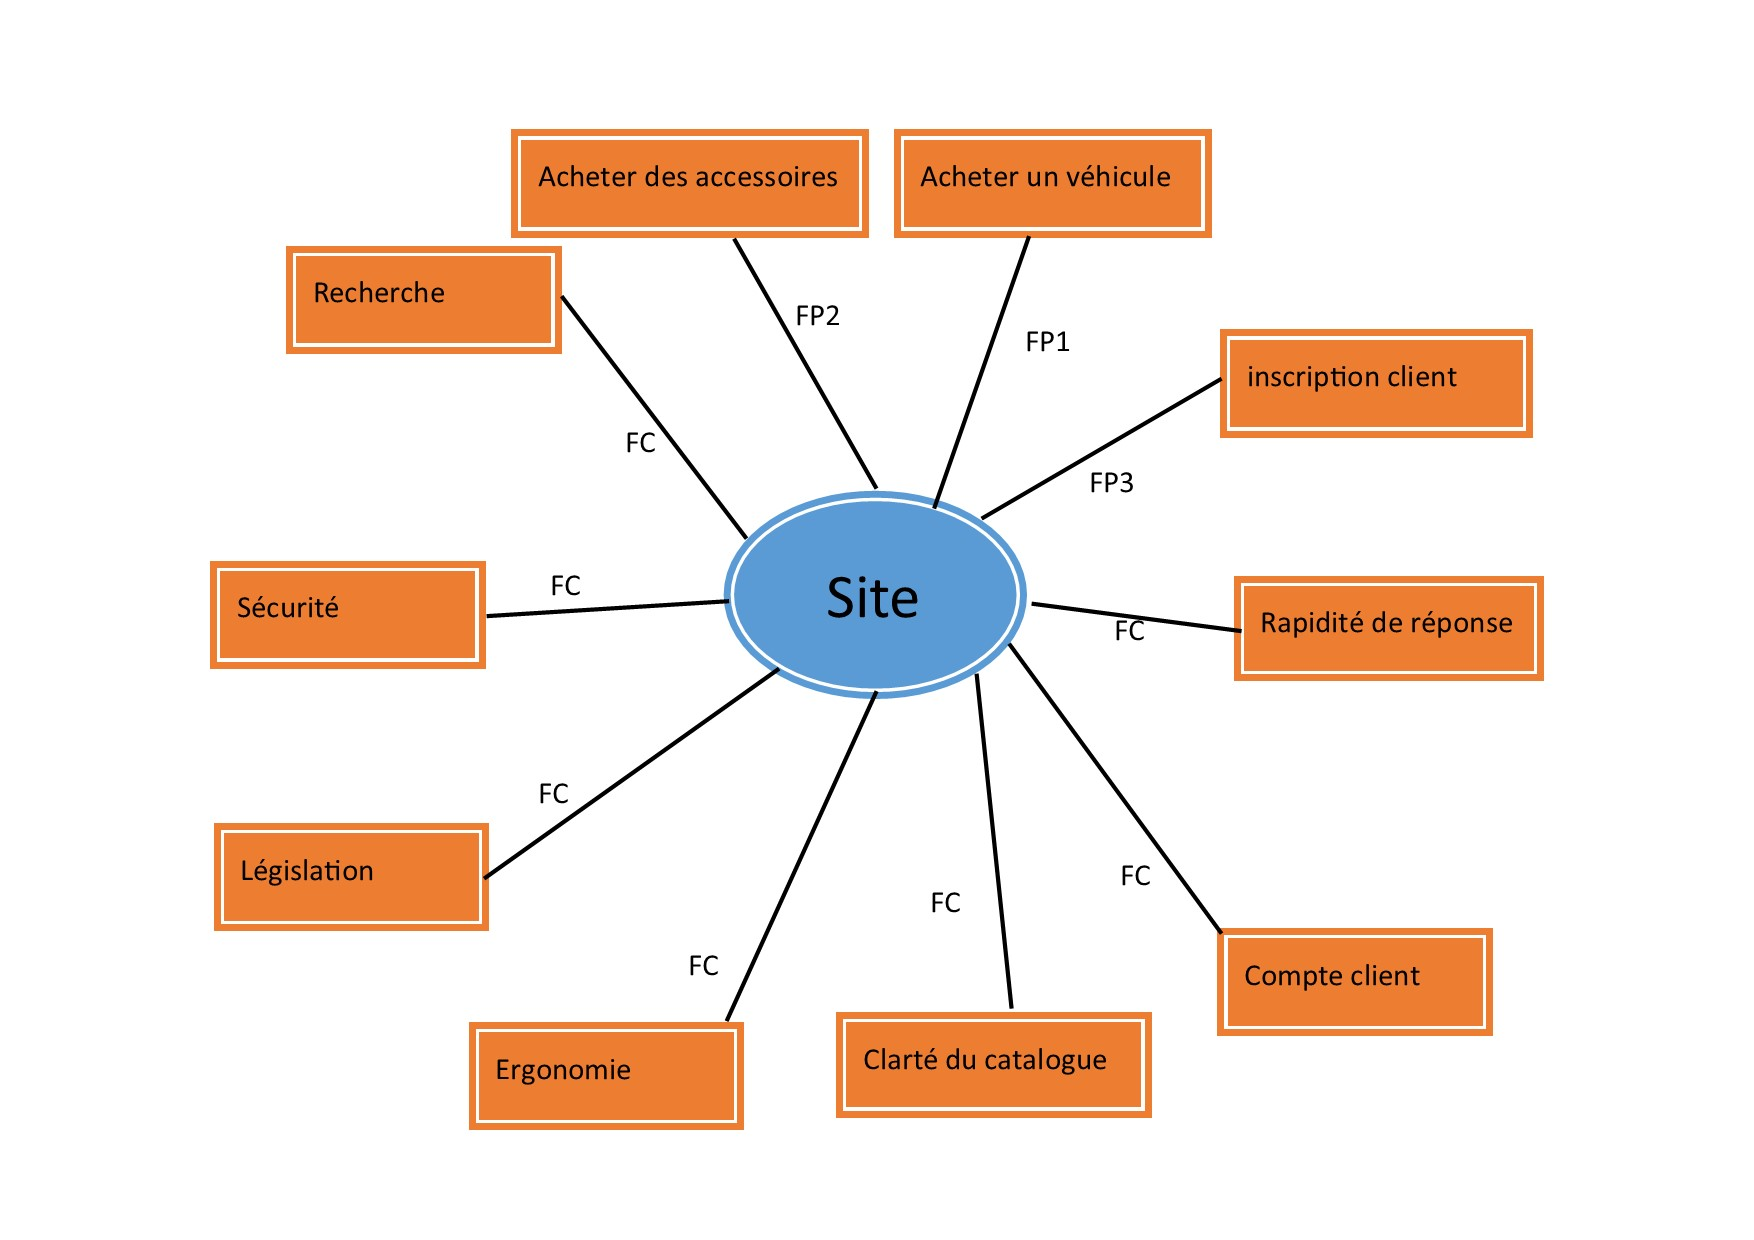
\includegraphics[scale=0.5]{../graph/pieuvre.jpg}
			\caption{Pieuvre de l'analyse fonctionnelle}
	\end{figure}
	\end{itemize}
	\subsection{Spécifications techniques et de réalisation}
	Pour réaliser ce projet, nous allons utiliser :
	\begin{itemize}
		\item[-] HTML, CSS, JavaScript et php pour l'implémentation du site;
		\item[-] Xamp pour faire le lien entre Apache, MySQL et php;
		\item[-] C++ sous Qt pour la réalisation de l'application
		\item[-] Gantt, outil de planification de projet;
	\end{itemize}

	\subsection{Gestion de projet}
	...
	
	\newpage
	\appendix
	\listoffigures
		
\end{document}